\title{Warm-Up for March 2nd, 2022}
\author{Dr. Jordan Hanson - Whittier College Dept. of Physics and Astronomy}
\date{\today}
\documentclass[12pt]{article}
\usepackage[a4paper, total={18cm, 27cm}]{geometry}
\usepackage{graphicx}
\usepackage{amsmath}
\usepackage{bm}
\begin{document}
\maketitle

\section{Memory Bank}

\begin{enumerate}
\item 2D charge density: $\sigma = Q/A$, where $Q$ and $A$ are the total charge and area, respectively
\item Laplace's Equation in 3D: $\nabla^2 V(\mathbf{r}) = 0$
\item Laplace's Equation in 1D: 
\begin{equation}
\frac{d^2 V}{dx^2} = 0
\end{equation}
\end{enumerate}

\begin{figure}[ht]
\centering
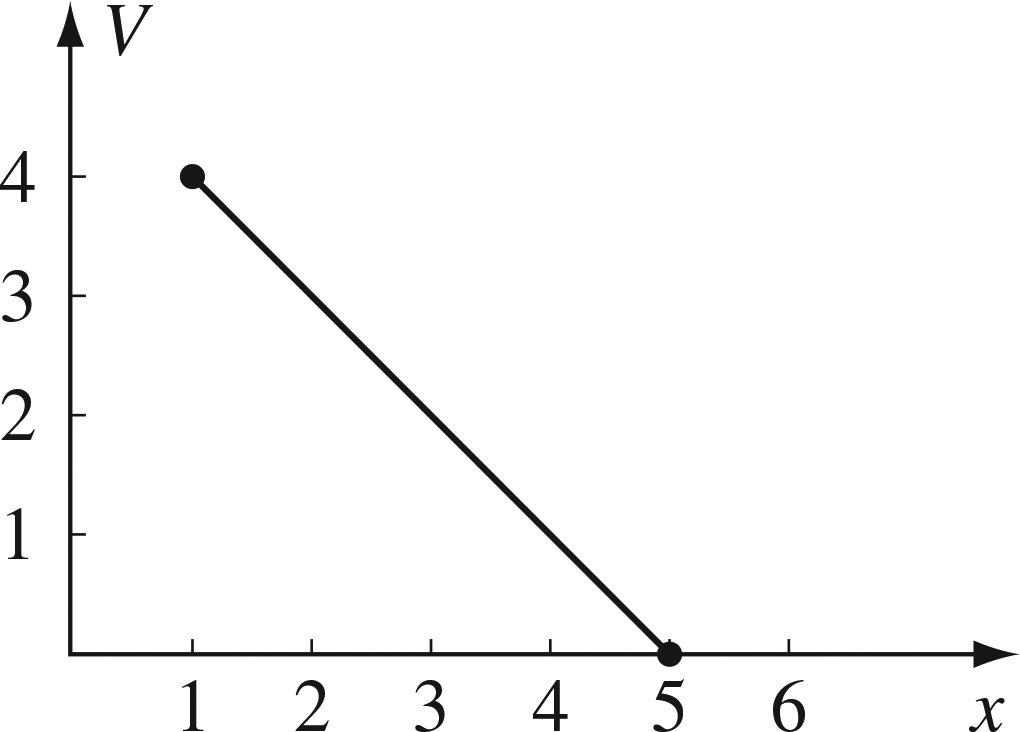
\includegraphics[width=0.2\textwidth]{figures/3_1.jpg}
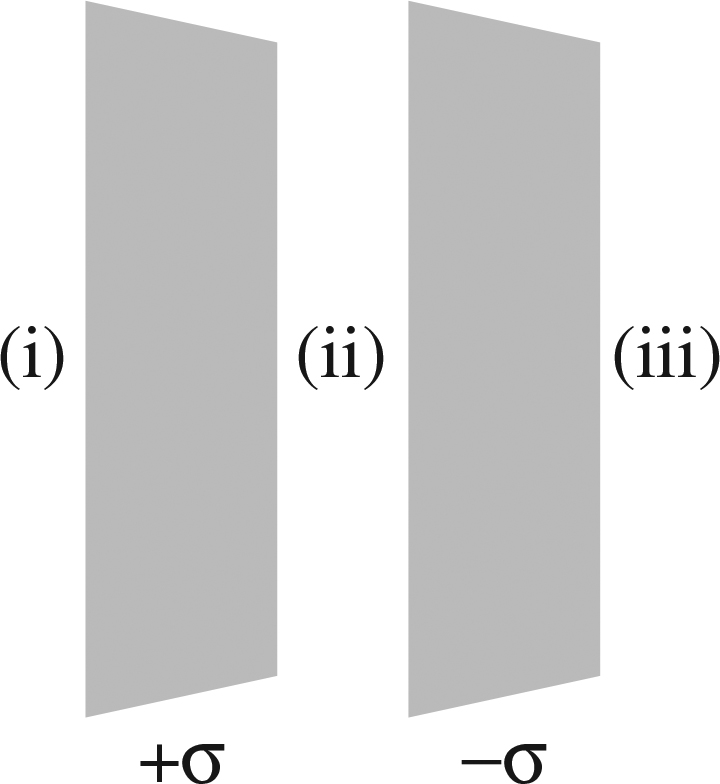
\includegraphics[width=0.2\textwidth]{figures/2_23.jpg}
\caption{\label{fig:f} (Left) A solution to \textit{Laplace's Equation} in 1D.  (Right) a 1D capacitor.}
\end{figure}

\section{Electric Field in a Parallel-Plate Capacitor}

Recall that the field near a flat plane of charge oriented in the $yz$-plane (see Fig. \ref{fig:f}, right) is 

\begin{equation}
\mathbf{E} = \frac{\sigma}{2\epsilon_0}\hat{x}
\end{equation}

\begin{itemize}
\item Show that for oppositely charged flat planes, the field is $\mathbf{E} = (\sigma/\epsilon_0) \hat{x}$ \\ \\
\item Note that $\mathbf{E}$ is a constant.  Suppose the negative side of the capacitor is grounded ($V = 0$), and the negative side is located at $x = 5$ mm.  Suppose the positive side is located at $x = 1$ mm, and has a potential of 4 Volts.  (a) Show that Fig. \ref{fig:f} (left) is the solution for $V(x)$ by solving Laplace's Equation. (b) In terms of given variables, what is the slope? (c) Show that $V(x)$ in the middle is the average of $V(x)$ at the endpoints.
\end{itemize}

\end{document}